\documentclass[twoside,twocolumn]{article}
\usepackage{blindtext} % Package to generate dummy text throughout this template 
\usepackage{graphicx}
\usepackage[sc]{mathpazo} % Use the Palatino font
\usepackage[T1]{fontenc} % Use 8-bit encoding that has 256 glyphs
\linespread{1.05} % Line spacing - Palatino needs more space between lines
\usepackage{microtype} % Slightly tweak font spacing for aesthetics

\usepackage[english]{babel} % Language hyphenation and typographical rules

\usepackage[hmarginratio=1:1,top=32mm,columnsep=20pt]{geometry} % Document margins
\usepackage[hang, small,labelfont=bf,up,textfont=it,up]{caption} % Custom captions under/above floats in tables or figures
\usepackage{booktabs} % Horizontal rules in tables

\usepackage{lettrine} % The lettrine is the first enlarged letter at the beginning of the text

\usepackage{enumitem} % Customized lists
\setlist[itemize]{noitemsep} % Make itemize lists more compact

\usepackage{abstract} % Allows abstract customization
\renewcommand{\abstractnamefont}{\normalfont\bfseries} % Set the "Abstract" text to bold
\renewcommand{\abstracttextfont}{\normalfont\small\itshape} % Set the abstract itself to small italic text

\usepackage{titlesec} % Allows customization of titles


\usepackage{fancyhdr} % Headers and foote
\pagestyle{fancy} % All pages have headers and footers
\fancyhead{} % Blank out the default header
\fancyfoot{} % Blank out the default footer
\fancyfoot[RO,LE]{\thepage} % Custom footer text

\usepackage{titling}

\usepackage{hyperref} 



\begin{document}

\title{ISO/IEC 9075:2008 standard of 2008}
\author{Angel Gonzales Cave}
\date {14 de agosto del 2019}
\maketitle

\begin{abstract}
En el presente artículo se explica las nuevas caracteristicas de la revision SQL:2008 para la estándar ISO para el lenguaje de consulta de la base de datos SQL, las características son  explicadas de forma sencilla y dando un ejemplo cuando es útil implementarlas en un ambiente real.
\end{abstract}
\begin{abstract}
This article explains the new features of the SQL revision: 2008 for the ISO standard for the query language of the SQL database, the characteristics are explained in a simple way and giving an example when it is useful to implement them in a real environment .
\end{abstract}

\section{Introducción}
Son muchas las revisiones que se publican para el estándar ISO para el lenguaje de bases de datos SQL. En este artículo se tratará sobre la revisión SQL:2008 donde se dará a conocer las nuevas funciones o caracterísiticas que trae la revisión en mención. Las funciones estarán enteramente descritas explicando los beneficios y en que casos podemos hacer empleo de las funciones.
\section{Marco Teórico}
\begin{itemize}
\item SQL(Lenguaje de Consulta Estructurada) es un lenguaje de programación estándar e interactivo para la obtención de información desde una base de datos y para actualizarla.
\item Script es un programa, o sea un conjunto de comandos, que se le da a un motor SQL para decirle lo que debe hacer y en que orden debe hacerlo.
\item Tabla se refiere al tipo de modelado de datos donde se guardan los datos recogidos por un programa.
\item Servidor basado en software es un programa que ofrece un servicio especial que otros programas denominados clientes pueden usar a nivel local o a través de una red.
\end{itemize}
\section{Análisis}
Las nuevas funciones son :
\begin{itemize}
\item Mejora de la instrucción MERGE esta sentencia permite actualizar una tabla objetivo basándose en el resultado de una unión con una tabla fuente. Es decir, puedo mantener actualizada una tabla en base a la información exigente en otra tabla, siempre y cuando las dos tengan un dato en común, como un código.

Esta tarea facilita el mantenimiento de tablas de tipo maestro cuando la información se obtiene de diferentes fuentes o de fuentes externas. Siendo esta instrucción la que utilizamos para lo que habitualmente hacemos al digitar nuestros scripts por ejemplo (Insert, Update o Delete), en donde tendriamos que realizar tres sentencias provocando un uso mayor de los recursos del servidor. Con MERGE nos permite hacer todo esto en una sola sentencia, lo que es mucho más eficiente y además se hará menor uso de los recursos del servidor.
El efecto que se quiere lograr es que en una sola sentencia se puedan realizar varias aciones. Típicamente esto implica:
\begin{itemize}
\item Actualizar datos
\item Insertar datos
\item Eliminar datos
\end{itemize}

\item TRUNCATE TABLE este comando se utiliza para eliminar o borrar los registros que se encuentren almacenados en una tabla. Este comando es util cuando se trabaja con tablas con registros temporales que no requieren ser almacenados en una tabla durante un largo periodo de tiempo.
Sentencia TRUNCATE TABLE :

\begin{center}
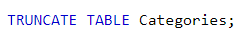
\includegraphics[width=7cm]{./Imagenes/01} 
\end{center}
\item Los triggers son disparadores los cuales nos ayuda a mantener la integridad de los datos mediante alertas que pueden implementarse en diferentes eventos.
 
Un INSTEAD OF trigger es un disparador que le permite saltar de una INSERT, DELETE o UPDATE comunicado a una tabla o una vista y ejecutar otros estados definidos en el gatillo en su lugar.

Un ejemplo típico de uso de un INSTEAD OF trigger es anular una operación de inserción, actualización o eliminación en una vista.

\begin{center}
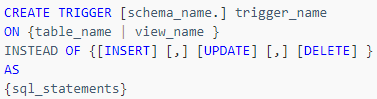
\includegraphics[width=7cm]{./Imagenes/02} 
\end{center}

\end{itemize}
\section{Conclusiones}
El uso de la instrucciión MERGE favorece en la optimización de la base de datos , donde los resultados se verán al realizar consultas en menor tiempo y haciendo menor uso de los recursos del servidor.

El comando TRUNCATE TABLE , este comando deja vacía una tabla , pero la tabla se mantiene ; es útil en tablas con registros temporales que no requieren ser almacenados por mucho tiempo.

Un INSTEAD OF trigger nos envia alertas omitiendo instrucciones DML y ejecutando otras instrucciones que estén definidas en la sentencia.

\begin{thebibliography}{}
\bibitem {}
\newblock en.wikipedia.org/wiki/SQL:2008
\bibitem {}
\newblock en.wikipedia.org/wiki/Merge(SQL)
\bibitem {}
\newblock sql.11sql.com/sql-truncate.html
\end{thebibliography}


\end{document}